\documentclass[journal]{IEEEtran}
\usepackage{iftex}
\ifPDFTeX
  \usepackage[utf8]{inputenc}
  \usepackage[T1]{fontenc}
\else
  \usepackage{fontspec}
  \setmainfont{texgyretermes}[Extension=.otf, UprightFont=*-regular, BoldFont=*-bold,
    ItalicFont=*-italic, BoldItalicFont=*-bolditalic]
\fi
\usepackage[spanish,es-tabla,es-nodecimaldot,es-noshorthands]{babel}
\usepackage{amsmath,amssymb}
\usepackage{graphicx}
\usepackage{booktabs}
\usepackage{multirow}
\usepackage{array}
\usepackage{url}
\usepackage{cite}
\graphicspath{{figuras/}}

\begin{document}

\title{Predicción de la Producción Diaria de Petróleo, Gas y Agua en el Campo Volve mediante un Ensemble de Modelos de Árboles}

\author{Carlos~Flores, Leonardo~de~Casanova y~Miguel~Ángel~Mori%
\thanks{Los autores pertenecen a la Universidad de Ingeniería y Tecnología (UTEC), Lima, Perú.}%
\thanks{Código y notebooks: \protect\url{https://github.com/Los-1000/machine-learning-final}.}}

\markboth{Proyecto Final de Machine Learning, noviembre~2026}%
{Flores \MakeLowercase{\textit{et al.}}: Predicción de producción en el campo Volve}

\maketitle

\begin{abstract}
Se presenta un modelo para predecir la producción diaria de petróleo (\texttt{BORE\_OIL\_VOL}), gas (\texttt{BORE\_GAS\_VOL}) y agua (\texttt{BORE\_WAT\_VOL}) de los pozos productores del campo Volve, cuyos datos fueron liberados públicamente por Equinor. A partir de las 34 variables disponibles se seleccionaron las mediciones operativas con significado físico, se construyó el historial reciente de cada pozo y se incorporó el volumen de agua inyectada en el campo. El modelo final es un ensemble que promedia LightGBM, Random Forest y Extra Trees. Cada modelo predice el cambio logarítmico de la producción respecto al día anterior, lo que evita el problema de extrapolación de los árboles de decisión. Con una validación temporal estricta (último 20\,\% de la vida de cada pozo), el ensemble alcanza $R^2$ entre 0.976 y 0.985 y un SMAPE entre 4.25\,\% y 4.57\,\% en los tres fluidos. Cumple así los requisitos de $R^2>0.9$ y SMAPE$<10$\,\% y supera a la línea base de persistencia.
\end{abstract}

\begin{IEEEkeywords}
Ingeniería de petróleo, pronóstico de producción, campo Volve, ensemble learning, LightGBM, Random Forest, Extra Trees, series de tiempo.
\end{IEEEkeywords}

\section{Introducción}
\IEEEPARstart{L}{a} predicción de la producción de hidrocarburos es esencial para planificar la operación de un campo petrolero, optimizar la inyección de agua y anticipar la irrupción de agua en los pozos. Los métodos clásicos, como el análisis de curvas de declinación o la simulación numérica de yacimientos, requieren supuestos fuertes o modelos geológicos costosos. Los métodos de aprendizaje automático, en cambio, pueden aprender directamente de los datos de sensores registrados en superficie y en el fondo del pozo.

En 2018, Equinor publicó el conjunto completo de datos del campo Volve, ubicado en el Mar del Norte y en producción entre 2008 y 2016~\cite{equinor}. Este trabajo usa los datos diarios de producción para construir un modelo que estime, para cada pozo productor y cada día, los volúmenes de petróleo, gas y agua. El modelo debe cumplir dos requisitos: un error porcentual absoluto medio simétrico (SMAPE) menor a 10 y un coeficiente de determinación $R^2$ mayor a 0.9.

\section{Descripción de los datos}
\subsection{Fuente y estructura}
El archivo \textit{Volve production data.xlsx} contiene dos hojas, con un total de 34 variables:
\begin{itemize}
\item \textbf{Hoja diaria:} 15\,634 registros y 24 variables.
\item \textbf{Hoja mensual:} 527 registros y 10 variables, que son agregados mensuales de la misma información.
\end{itemize}
Las variables objetivo son \texttt{BORE\_OIL\_VOL}, \texttt{BORE\_GAS\_VOL} y \texttt{BORE\_WAT\_VOL}. La fecha se registra en \texttt{DATEPRD}. Cada pozo se identifica con \texttt{WELL\_BORE\_CODE} y \texttt{NPD\_WELL\_BORE\_NAME}, y su tipo se indica con \texttt{FLOW\_KIND} y \texttt{WELL\_TYPE}.

\subsection{Tipos de pozo}
El campo cuenta con siete pozos:
\begin{itemize}
\item \textbf{Cinco productores} (\texttt{WELL\_TYPE}=OP): F-1~C, F-11, F-12, F-14 y F-15~D.
\item \textbf{Dos inyectores de agua} (\texttt{WELL\_TYPE}=WI): F-4 y F-5. Mantienen la presión del yacimiento. El pozo F-5 operó brevemente como productor antes de su conversión.
\end{itemize}
Los inyectores no producen fluidos, por lo que sus variables objetivo son nulas. Su única variable propia es el volumen inyectado, \texttt{BORE\_WI\_VOL}.

\subsection{Análisis exploratorio}
La Fig.~\ref{fig:pozos} muestra la producción diaria de cada pozo y la Fig.~\ref{fig:balance}, el balance del campo completo. La producción de petróleo alcanza su máximo en 2009 y luego declina. Al mismo tiempo, el agua producida crece de forma sostenida a partir de 2010, impulsada por la inyección de agua. Este aumento del corte de agua con el tiempo implica que el comportamiento futuro de los pozos no está bien representado en el pasado, lo que dificulta la extrapolación.

En el análisis exploratorio también se encontraron problemas de calidad en los datos:
\begin{itemize}
\item 1\,132 días productores con \texttt{ON\_STREAM\_HRS}=0, es decir, con el pozo cerrado.
\item 2\,311 lecturas nulas de presión de fondo, que corresponden a sensores fuera de servicio.
\item 4 volúmenes de agua negativos, físicamente imposibles.
\end{itemize}

\begin{figure*}[!t]
\centering
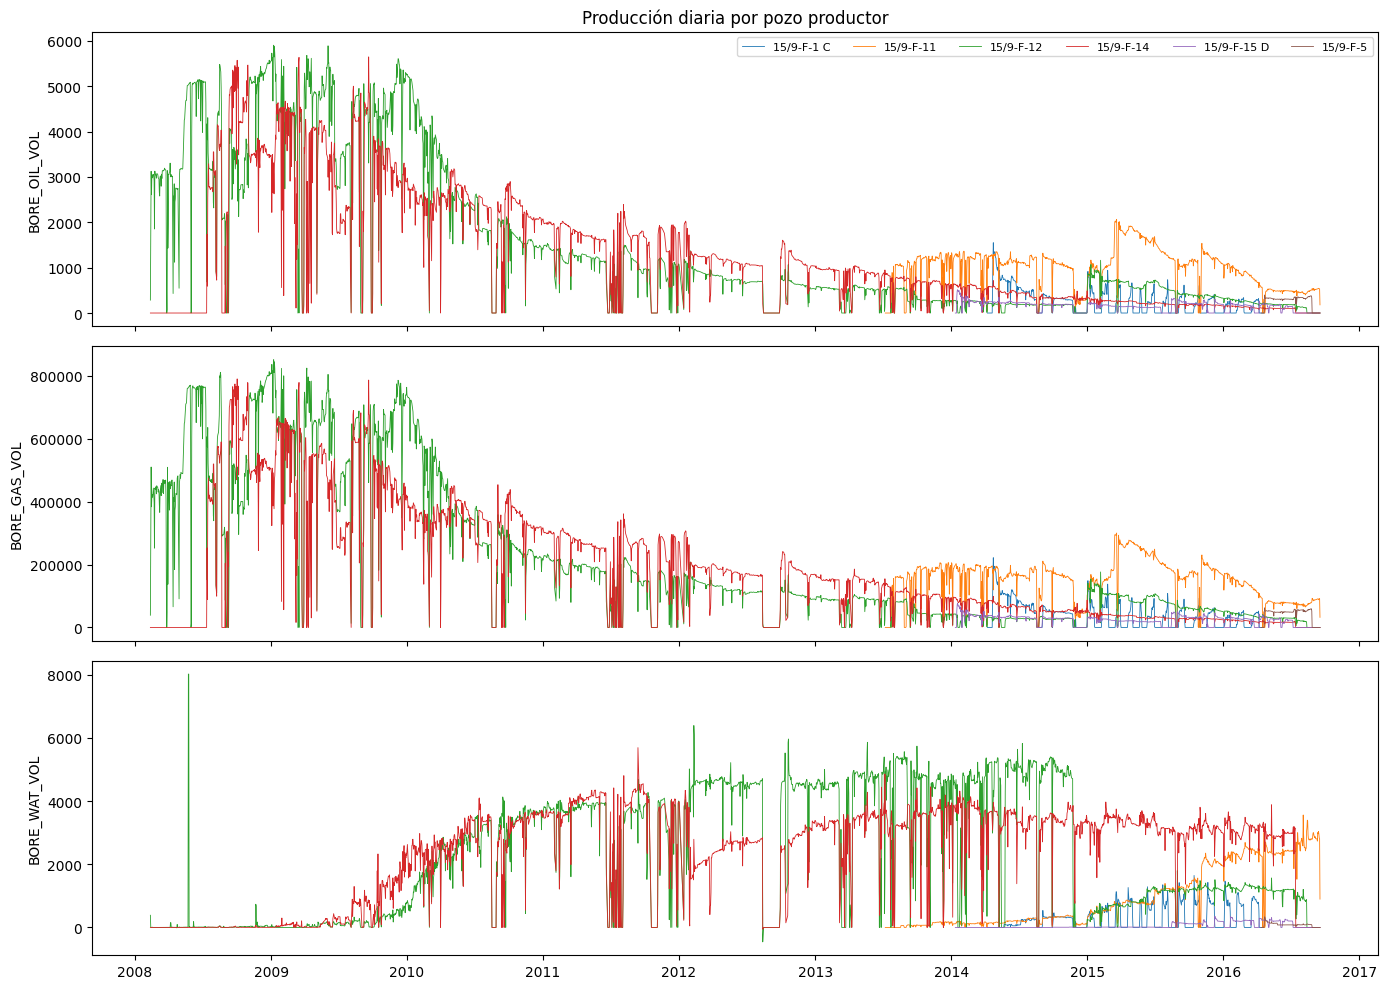
\includegraphics[width=0.92\textwidth]{produccion_por_pozo.png}
\caption{Producción diaria de petróleo, gas y agua por pozo productor (2008--2016).}
\label{fig:pozos}
\end{figure*}

\begin{figure}[!t]
\centering
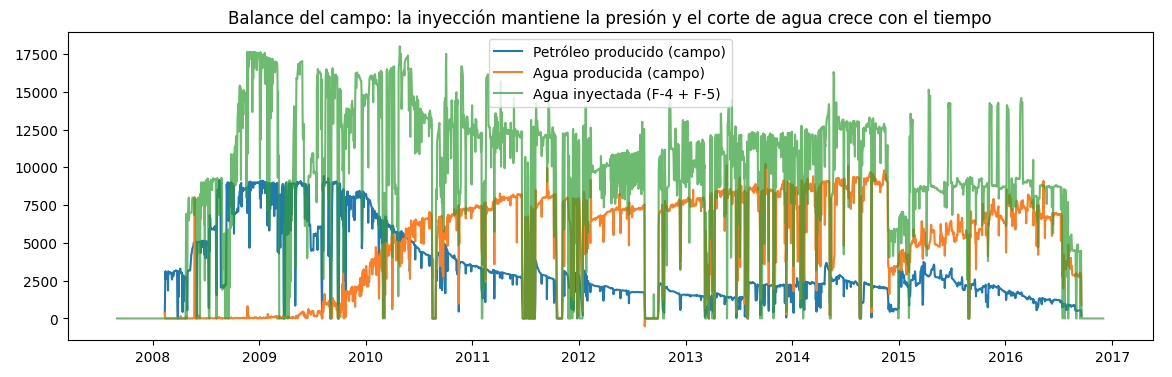
\includegraphics[width=\columnwidth]{balance_campo.png}
\caption{Balance del campo: petróleo producido, agua producida y agua inyectada por los pozos F-4 y F-5. La inyección sostiene la presión y el corte de agua aumenta con el tiempo.}
\label{fig:balance}
\end{figure}

\section{Metodología}
\subsection{Selección de variables}
La Tabla~\ref{tab:vars} resume qué se hizo con cada grupo de variables.
\begin{itemize}
\item \textbf{Descartadas:} las constantes (códigos de campo y plataforma, unidad del estrangulador), los identificadores (se usan solo para agrupar) y la hoja mensual (es redundante).
\item \textbf{Filtro:} \texttt{FLOW\_KIND} y \texttt{WELL\_TYPE} se usan para quedarse solo con los registros de pozos productores.
\item \textbf{Inyección:} \texttt{BORE\_WI\_VOL} de los inyectores no se descarta. Se agrega por día para formar la variable \texttt{INY\_CAMPO}, que representa el soporte de presión que recibe todo el yacimiento.
\end{itemize}

\begin{table}[!t]
\centering
\caption{Selección de variables}
\label{tab:vars}
\footnotesize
\begin{tabular}{>{\raggedright\arraybackslash}p{3.3cm}>{\raggedright\arraybackslash}p{1.4cm}>{\raggedright\arraybackslash}p{2.7cm}}
\toprule
\textbf{Variable(s)} & \textbf{Uso} & \textbf{Motivo}\\
\midrule
Códigos/nombres de campo e instalación, \texttt{AVG\_CHOKE\_UOM} & Descartada & Constantes\\
\texttt{WELL\_BORE\_CODE}, \texttt{NPD\_WELL\_BORE\_*} & Agrupación & Identificadores\\
\texttt{FLOW\_KIND}, \texttt{WELL\_TYPE} & Filtro & Solo productores (OP)\\
\texttt{DATEPRD} & Orden y partición & Fecha\\
Horas en línea, presiones y temperaturas de fondo y cabeza, $\Delta P$ tubing, presión anular, estrangulador & Entrada & Controlan físicamente el caudal\\
\texttt{BORE\_WI\_VOL} & Entrada agregada & Inyección del campo\\
\texttt{BORE\_*\_VOL} (días previos) & Entrada & Historial del pozo\\
Hoja mensual & Descartada & Redundante\\
\bottomrule
\end{tabular}
\end{table}

\subsection{Limpieza}
Se modelan únicamente los días con el pozo en operación (\texttt{ON\_STREAM\_HRS}$>0$) y con volúmenes positivos. Esto deja 7\,499 registros.

Los días con el pozo cerrado no necesitan modelo: se resuelven con la regla \emph{producción = 0}. Además, el SMAPE no está definido cuando tanto el valor real como la predicción son nulos, por lo que esos días no pueden evaluarse con esa métrica.

Los valores faltantes de los sensores se tratan así:
\begin{itemize}
\item LightGBM los maneja de forma nativa.
\item En los bosques aleatorios se imputan con $-1$, un valor fuera del rango físico que los árboles aprenden a separar.
\end{itemize}

\subsection{Ingeniería de variables}
Para cada pozo, y usando solo información de días anteriores (sin fuga de información), se construyeron 37 variables de entrada:
\begin{itemize}
\item \textbf{Historial de producción:} rezagos de 1, 2 y 7 días y media móvil de 7 días de cada fluido.
\item \textbf{Cambios operativos diarios ($\Delta$):} de las horas en línea, la presión en cabeza, la apertura del estrangulador, la presión de fondo y $\Delta P$ del estrangulador.
\item \textbf{Relaciones de fluidos del día anterior:} corte de agua y relación gas-petróleo (GOR).
\item \textbf{Inyección del campo:} volumen inyectado en el día y su media de 7 días.
\item \textbf{Otras:} antigüedad del pozo en días y código del pozo.
\end{itemize}

\subsection{Transformación del objetivo}
Los modelos basados en árboles predicen valores constantes por tramos, así que no pueden extrapolar a niveles que no vieron durante el entrenamiento. Esto es crítico para el agua, cuyo volumen crece en el tiempo (Fig.~\ref{fig:balance}). Por eso cada modelo aprende el cambio logarítmico respecto al día anterior:
\begin{equation}
z_t = \ln(1+y_t) - \ln(1+y_{t-1}),
\end{equation}
y la predicción se reconstruye como
\begin{equation}
\hat{y}_t = \exp\!\big(\ln(1+y_{t-1}) + \hat{z}_t\big) - 1 .
\end{equation}

\subsection{Modelos y ensemble}
Para cada variable objetivo se entrenan tres regresores:
\begin{itemize}
\item \textbf{LightGBM}~\cite{lightgbm}: \textit{gradient boosting} con 1\,000 árboles, tasa de aprendizaje 0.02, 31 hojas y submuestreo de filas y columnas de 0.8.
\item \textbf{Random Forest}~\cite{breiman}: 400 árboles y un mínimo de 2 muestras por hoja.
\item \textbf{Extra Trees}~\cite{extratrees}: 400 árboles con umbrales de corte aleatorios.
\end{itemize}
El \emph{boosting} reduce principalmente el sesgo y el \emph{bagging}, la varianza. Por eso sus errores están poco correlacionados y su combinación los reduce~\cite{dietterich}.

La predicción final es el promedio simple de las tres:
\begin{equation}
\hat{y}^{\,ens}_t = \tfrac{1}{3}\big(\hat{y}^{\,LGB}_t + \hat{y}^{\,RF}_t + \hat{y}^{\,ET}_t\big).
\end{equation}
Como referencia se usa un modelo de persistencia, $\hat{y}_t = y_{t-1}$. La implementación usa scikit-learn~\cite{sklearn}.

\subsection{Validación y métricas}
Para simular un pronóstico real, los registros de cada pozo se ordenan cronológicamente. El 80\,\% inicial se usa para entrenar (5\,998 registros) y el 20\,\% final, para probar (1\,501 registros; desde 2015 hasta septiembre de 2016). Se reportan dos métricas~\cite{hyndman}:
\begin{equation}
\mathrm{SMAPE}=\frac{100}{n}\sum_{i=1}^{n}\frac{2\,|\hat{y}_i-y_i|}{|y_i|+|\hat{y}_i|},\qquad
R^2 = 1-\frac{\sum (y_i-\hat{y}_i)^2}{\sum (y_i-\bar{y})^2}.
\end{equation}

\section{Resultados}
La Tabla~\ref{tab:res} compara cada modelo en el conjunto de prueba. Sobre los modelos individuales:
\begin{itemize}
\item Random Forest y Extra Trees obtienen el mejor $R^2$ en petróleo y gas.
\item Extra Trees es el más preciso en agua.
\item LightGBM es el más débil por separado, pero aporta diversidad al ensemble.
\end{itemize}
El ensemble consigue el menor SMAPE en petróleo y gas, y en agua queda prácticamente empatado con el mejor modelo (Extra Trees).

\begin{table}[!t]
\centering
\caption{Resultados en el conjunto de prueba temporal}
\label{tab:res}
\footnotesize
\setlength{\tabcolsep}{3.5pt}
\begin{tabular}{lcccccc}
\toprule
& \multicolumn{2}{c}{\textbf{Petróleo}} & \multicolumn{2}{c}{\textbf{Gas}} & \multicolumn{2}{c}{\textbf{Agua}}\\
\textbf{Modelo} & $R^2$ & SMAPE & $R^2$ & SMAPE & $R^2$ & SMAPE\\
\midrule
Persistencia      & 0.947 & 6.25 & 0.946 & 6.30 & 0.953 & 6.13\\
LightGBM          & 0.970 & 6.17 & 0.962 & 6.93 & 0.972 & 5.94\\
Random Forest     & 0.980 & 4.84 & 0.981 & 4.85 & 0.975 & 6.45\\
Extra Trees       & 0.978 & 5.13 & 0.974 & 5.20 & 0.985 & 4.15\\
\textbf{Ensemble} & \textbf{0.978} & \textbf{4.44} & \textbf{0.976} & \textbf{4.57} & \textbf{0.985} & \textbf{4.25}\\
\midrule
Requisito & $>0.9$ & $<10$ & $>0.9$ & $<10$ & $>0.9$ & $<10$\\
\bottomrule
\end{tabular}
\end{table}

La Fig.~\ref{fig:scatter} compara los valores reales con los predichos: los puntos se concentran sobre la diagonal en los tres fluidos. La Fig.~\ref{fig:series} muestra que el ensemble sigue con precisión la tendencia de declinación y los eventos operativos (cierres y reaperturas) de los tres pozos principales.

Los errores más grandes aparecen el día en que un pozo se reabre después de un cierre parcial. En esos días el volumen del día anterior no es representativo, y el modelo depende de los cambios en las horas en línea.

\begin{figure*}[!t]
\centering
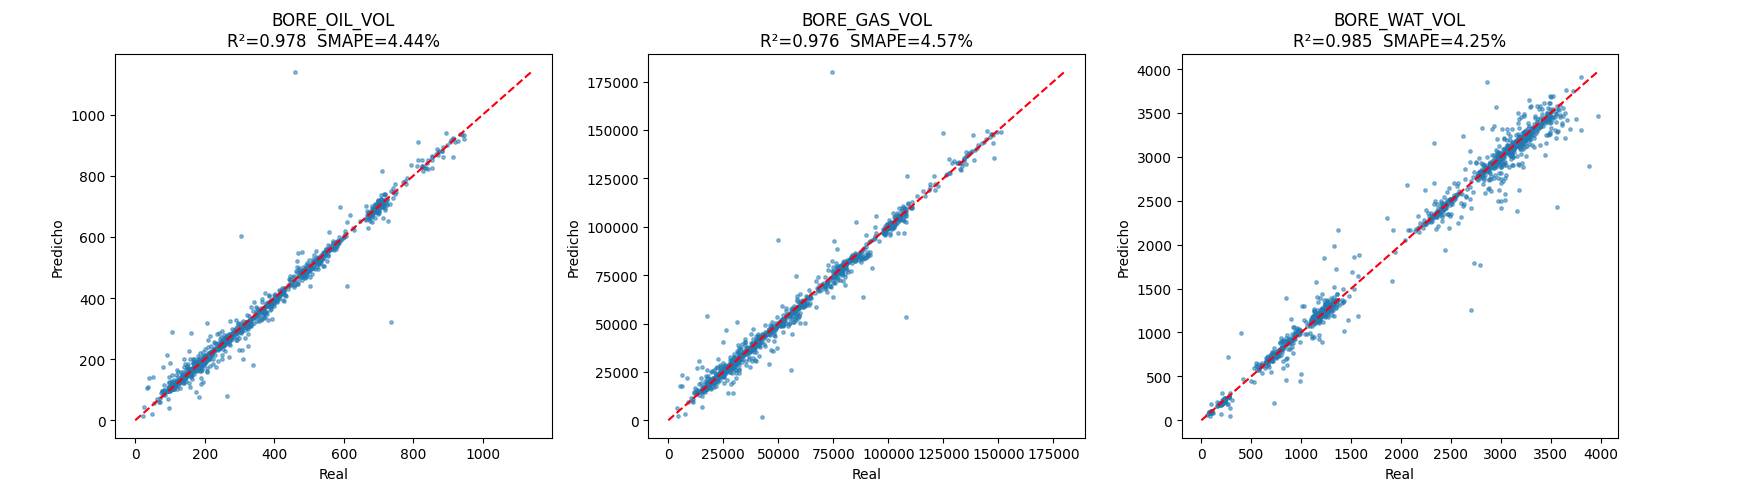
\includegraphics[width=0.95\textwidth]{real_vs_predicho.png}
\caption{Valores reales frente a valores predichos por el ensemble en el conjunto de prueba. La línea discontinua es la predicción perfecta.}
\label{fig:scatter}
\end{figure*}

\begin{figure*}[!t]
\centering
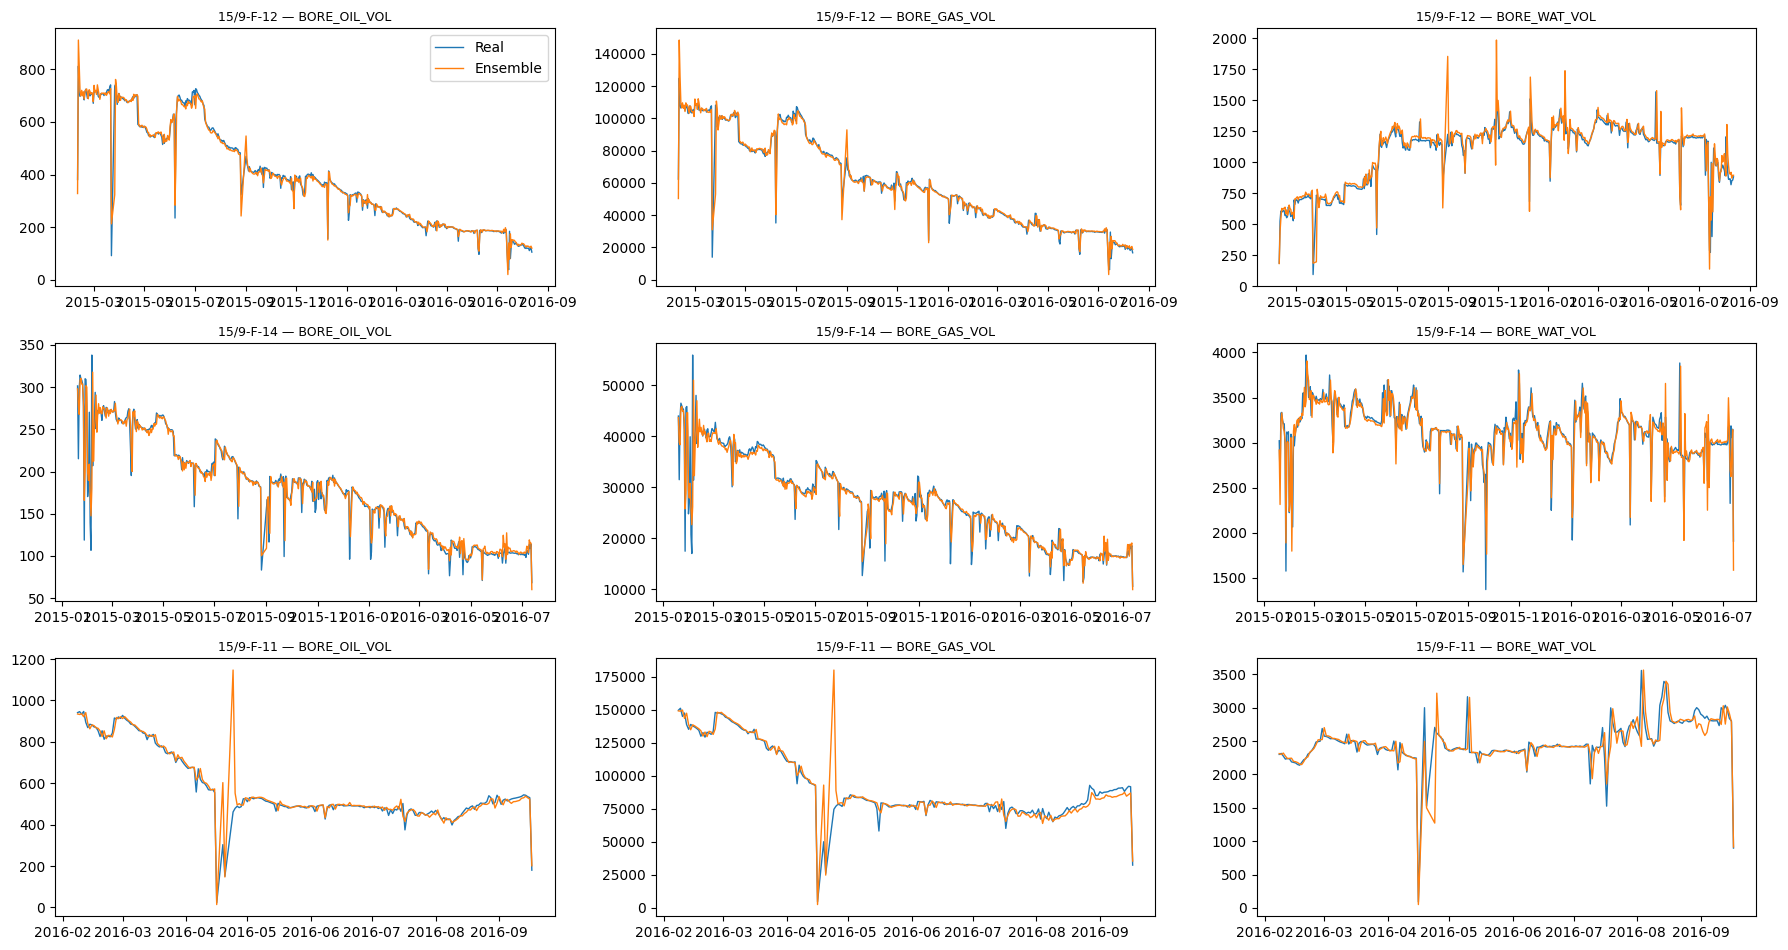
\includegraphics[width=0.95\textwidth]{series_test.png}
\caption{Series reales y predichas en el periodo de prueba para los pozos F-12, F-14 y F-11.}
\label{fig:series}
\end{figure*}

\subsection{Importancia de variables}
La Fig.~\ref{fig:imp} muestra la importancia de las variables según el Random Forest. Las dos más relevantes son la variación diaria de las horas en línea (\texttt{ON\_STREAM\_HRS\_diff}) y las propias horas en línea, lo cual es coherente con la física del problema. Como el objetivo es el cambio respecto al día anterior, el principal motivo de cambio es que el pozo haya operado más o menos horas.

Les siguen la producción del día anterior y los cambios en el estrangulador y en las presiones. En el caso del agua también pesan el corte de agua, la antigüedad del pozo y la inyección del campo, que reflejan el avance del frente de agua.

\begin{figure*}[!t]
\centering
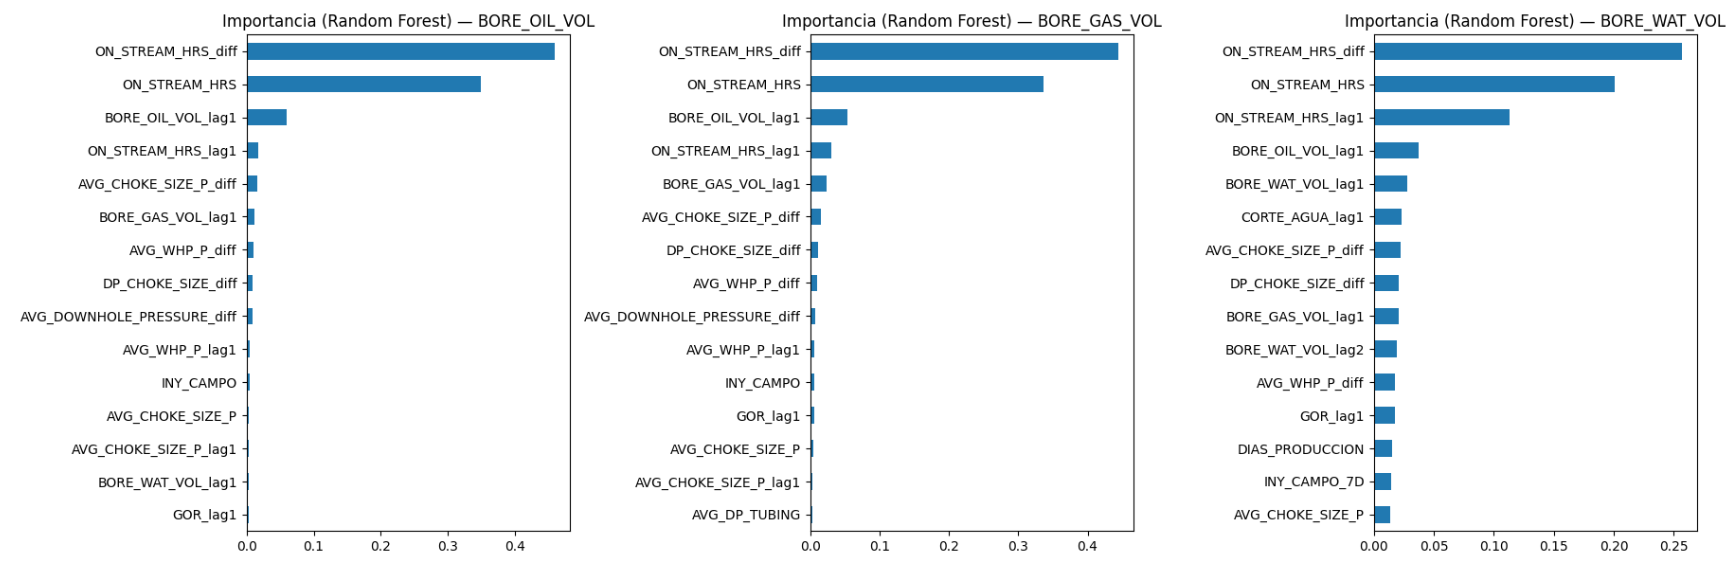
\includegraphics[width=0.95\textwidth]{importancia_variables.png}
\caption{Las 15 variables más importantes (Random Forest) para cada fluido.}
\label{fig:imp}
\end{figure*}

\subsection{Análisis por pozo}
En los pozos principales (F-11, F-12 y F-14), el SMAPE se mantiene entre 2.8\,\% y 4.4\,\%. El pozo F-1~C muestra errores mayores (alrededor del 13\,\% en petróleo y gas) por dos motivos: tiene solo 76 días de prueba y se encuentra al final de su vida productiva, con un comportamiento muy inestable.

\section{Discusión}
Formular el objetivo como el cambio respecto al día anterior fue la decisión clave. En un experimento preliminar que predecía el volumen absoluto, el modelo de agua alcanzó solo $R^2=0.72$, porque los árboles no podían extrapolar el aumento del corte de agua.

Que el ensemble supere a la persistencia demuestra que el modelo aporta información adicional a la inercia del pozo: un SMAPE de 4.3--4.6 frente a 6.1--6.3.

Este trabajo tiene dos limitaciones principales:
\begin{itemize}
\item \textbf{Horizonte de un día:} el modelo pronostica solo el día siguiente, porque necesita la producción del día anterior. Para horizontes más largos habría que usar predicción recursiva o modelos secuenciales (por ejemplo, LSTM).
\item \textbf{Validez del conjunto de prueba:} el conjunto de prueba pertenece al mismo campo. Generalizar el modelo a otros campos requeriría volver a entrenarlo.
\end{itemize}

\section{Conclusiones}
Se construyó un ensemble de LightGBM, Random Forest y Extra Trees que predice la producción diaria de petróleo, gas y agua del campo Volve. Con validación temporal y sin fuga de información, el modelo obtiene $R^2\geq 0.976$ y SMAPE$\leq 4.57$\,\% en los tres fluidos, y cumple holgadamente los requisitos planteados.

La selección de variables con criterio físico, la incorporación de la inyección del campo como variable explicativa y la transformación del objetivo fueron determinantes para el desempeño del modelo.

\begin{thebibliography}{9}
\bibitem{equinor} Equinor, ``Volve field data set,'' 2018. [Online]. Available: \url{https://www.equinor.com/energy/volve-data-sharing}
\bibitem{lightgbm} G. Ke \textit{et al.}, ``LightGBM: A highly efficient gradient boosting decision tree,'' in \textit{Proc. NeurIPS}, 2017, pp. 3146--3154.
\bibitem{breiman} L. Breiman, ``Random forests,'' \textit{Mach. Learn.}, vol. 45, no. 1, pp. 5--32, 2001.
\bibitem{extratrees} P. Geurts, D. Ernst, and L. Wehenkel, ``Extremely randomized trees,'' \textit{Mach. Learn.}, vol. 63, no. 1, pp. 3--42, 2006.
\bibitem{dietterich} T. G. Dietterich, ``Ensemble methods in machine learning,'' in \textit{Proc. Int. Workshop Multiple Classifier Systems}, 2000, pp. 1--15.
\bibitem{sklearn} F. Pedregosa \textit{et al.}, ``Scikit-learn: Machine learning in Python,'' \textit{J. Mach. Learn. Res.}, vol. 12, pp. 2825--2830, 2011.
\bibitem{hyndman} R. J. Hyndman and A. B. Koehler, ``Another look at measures of forecast accuracy,'' \textit{Int. J. Forecast.}, vol. 22, no. 4, pp. 679--688, 2006.
\end{thebibliography}

\end{document}
